\documentclass[tikz,border=5pt]{standalone}
\usepackage{tikz}
\usepackage{amsmath}
\usetikzlibrary{arrows.meta,angles,quotes}
\definecolor{nebula}{HTML}{6366F1}
\definecolor{spark}{HTML}{14B8A6}
\definecolor{ink}{HTML}{334155}
\begin{document}
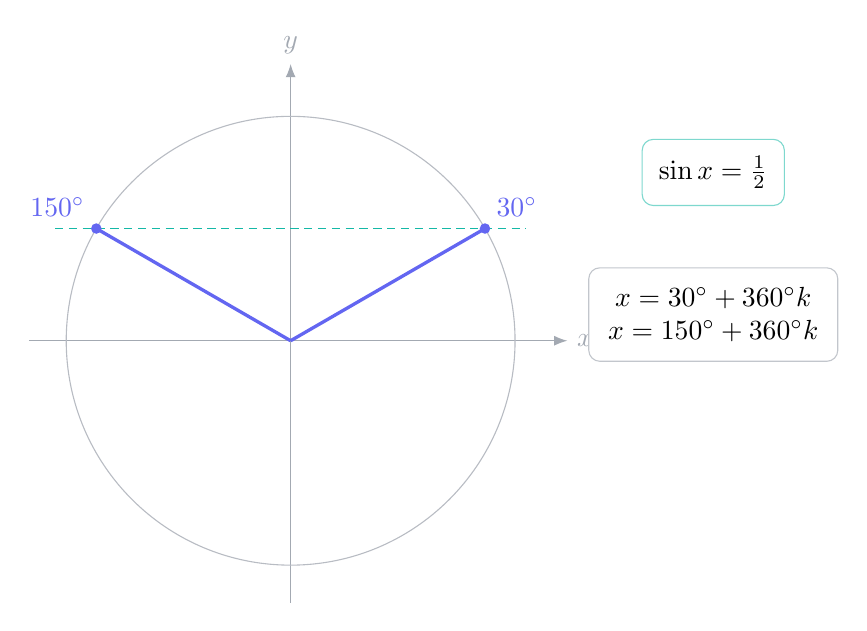
\begin{tikzpicture}[font=\sffamily,>=Latex,scale=.95]
  \draw[->,ink!45] (-3.5,0)--(3.7,0) node[right] {$x$};
  \draw[->,ink!45] (0,-3.5)--(0,3.7) node[above] {$y$};
  \draw[ink!35] (0,0) circle (3);
  \draw[densely dashed,spark] (-3.15,1.5)--(3.15,1.5);
  \coordinate (A) at (30:3);
  \coordinate (B) at (150:3);
  \fill[nebula] (A) circle (2pt) node[above right=3pt,fill=white,inner sep=1pt] {$30^\circ$};
  \fill[nebula] (B) circle (2pt) node[above left=3pt,fill=white,inner sep=1pt] {$150^\circ$};
  \draw[very thick,nebula] (0,0)--(A);
  \draw[very thick,nebula] (0,0)--(B);
  \node[draw=spark!55,rounded corners=4pt,fill=white,inner sep=6pt] at (5.65,2.25)
    {$\sin x=\tfrac12$};
  \node[draw=ink!30,rounded corners=4pt,fill=white,inner sep=7pt,align=center] at (5.65,.35)
    {$x=30^\circ+360^\circ k$\\$x=150^\circ+360^\circ k$};
\end{tikzpicture}
\end{document}
